\documentclass[../main.tex]{subfiles}

\graphicspath{{../images/}}

\begin{document}
\pagestyle{fancy}
\lhead{Homework 2}
\chead{Junseo Shin}
\rhead{PHYS 421}

\setcounter{section}{2}
% 2.2, 2.5, 2.7, 2.8, 2.12, 2.16, 2.18
\paragraph{2.2}
\begin{figure}[ht]
    \centering
    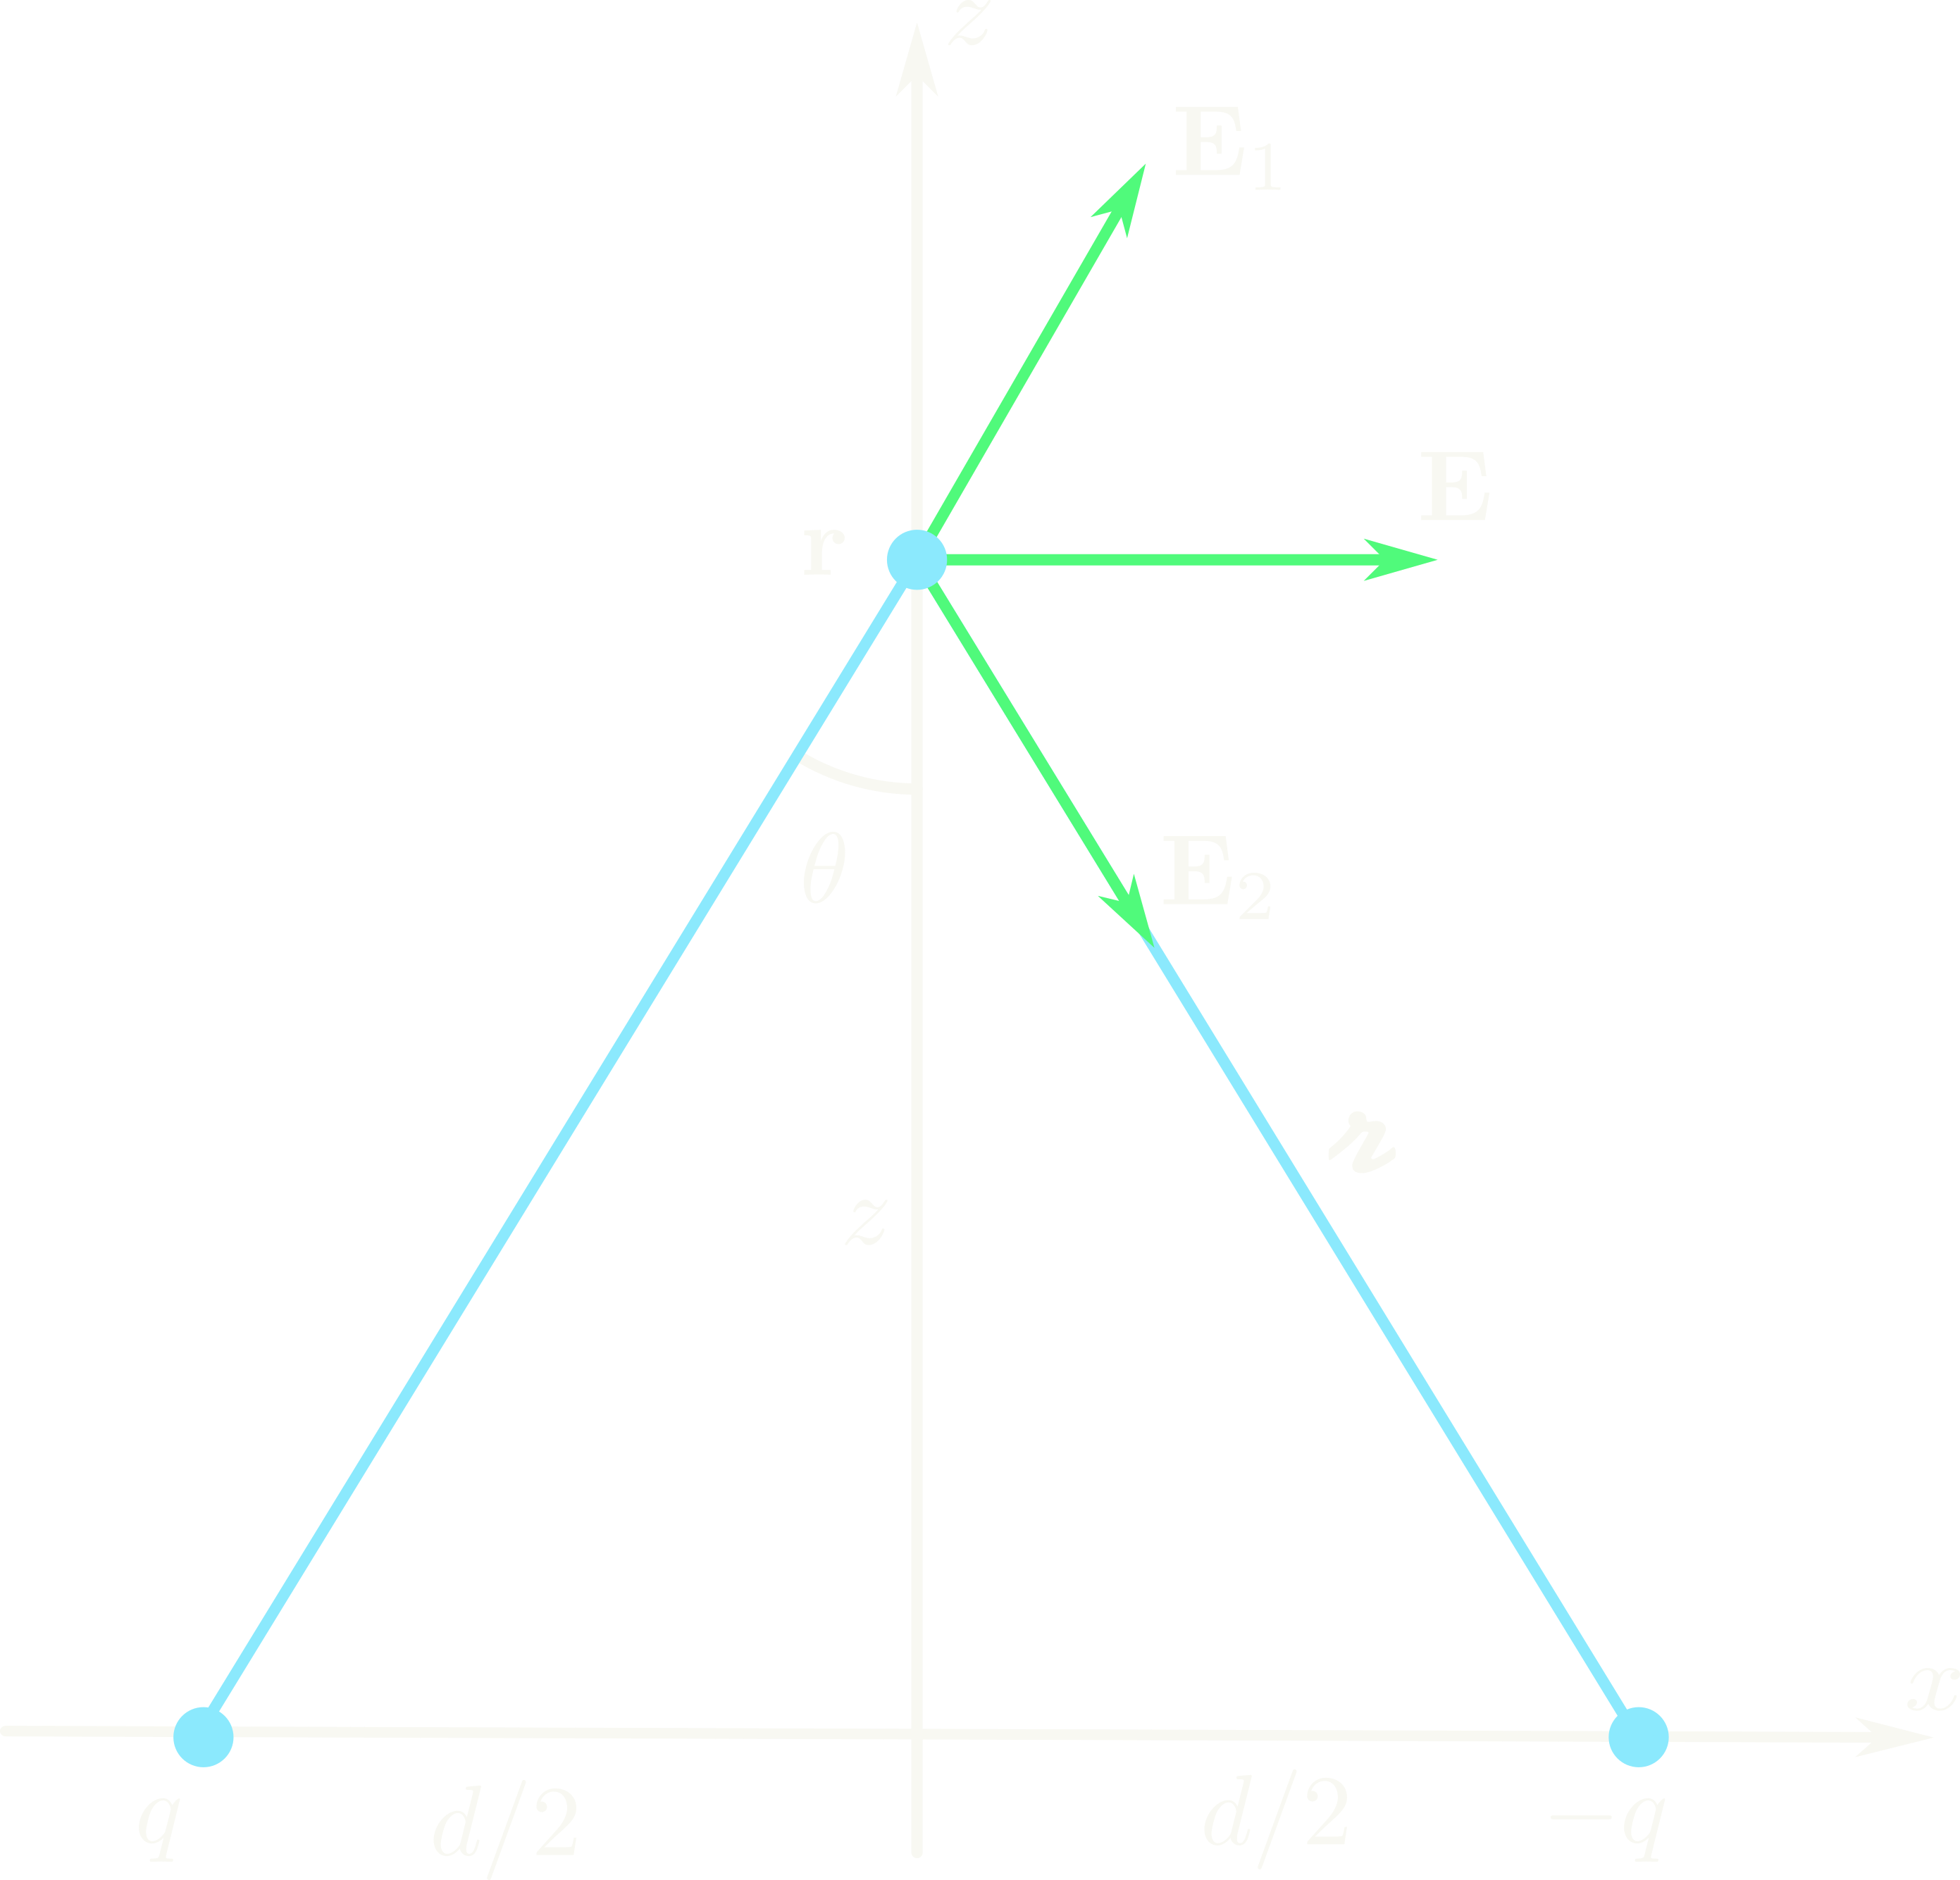
\includegraphics[width=0.5\linewidth]{images/hw2_2.png}
    \captionsetup{width=0.8\linewidth}
    \caption{An electric field at a distance $z$ from the midpoint between equal and opposite
    charges $(\pm q)$ separated by a distance $d$. The charge at $x = d/2$ is $-q$.}
    \label{fig:2_2}
\end{figure}
The vertical componets of the electric field cancel out and the horizontal components add up:
\begin{align*}
    E_x &= 2 \frac{1}{4\pi\epsilon_0} \frac{q}{\scriptr^2} \sin \theta
\end{align*}
where $E_x = E \cos \theta$, $\scriptr = \sqrt{z^2 + (d/2)^2}$, and $\sin \theta = d / (2\scriptr)$,
so 
\begin{align*}
    \vb{E} = \frac{1}{4\pi\epsilon_0} \frac{qd}{[z^2 + (d/2)^2]^{3/2}} \vu{x}
\end{align*}

\newpage
\paragraph{2.5}
The horizontal components of the electric field cancel out, and the vertical components conspire:
\begin{align*}
    \vb{E} &= \frac{1}{4\pi\epsilon_0}
        \int \frac{\lambda}{\scriptr^2} \cos\theta \vu{z} \dd{\vb{l}}
\end{align*}
where geometrically $\scriptr = \sqrt{z^2 + r^2}$ and $\cos\theta = z / \scriptr$. So,
\begin{align*}
    \vb{E} &= \frac{1}{4\pi\epsilon_0}
        \int \frac{\lambda z}{(z^2 + r^2)^{3/2}} \vu{z} \dd{\vb{l}}
\end{align*}
and the line integral is over the circumference of the circle, so $\dd{\vb{l}} = r \dd{\theta}$ and
the limits of integration are $[0, 2\pi]$:
\begin{align*}
    \vb{E} &= \frac{1}{4\pi\epsilon_0} \frac{\lambda z}{(z^2 + r^2)^{3/2}} \vu{z}
        \int_0^{2\pi}  r \dd{\theta} \\
    &= \frac{1}{4\pi\epsilon_0}
        \frac{\lambda z (2\pi r)}{(z^2 + r^2)^{3/2}}
\end{align*}

\newpage
\paragraph{2.7}
\begin{figure}[ht]
    \centering
    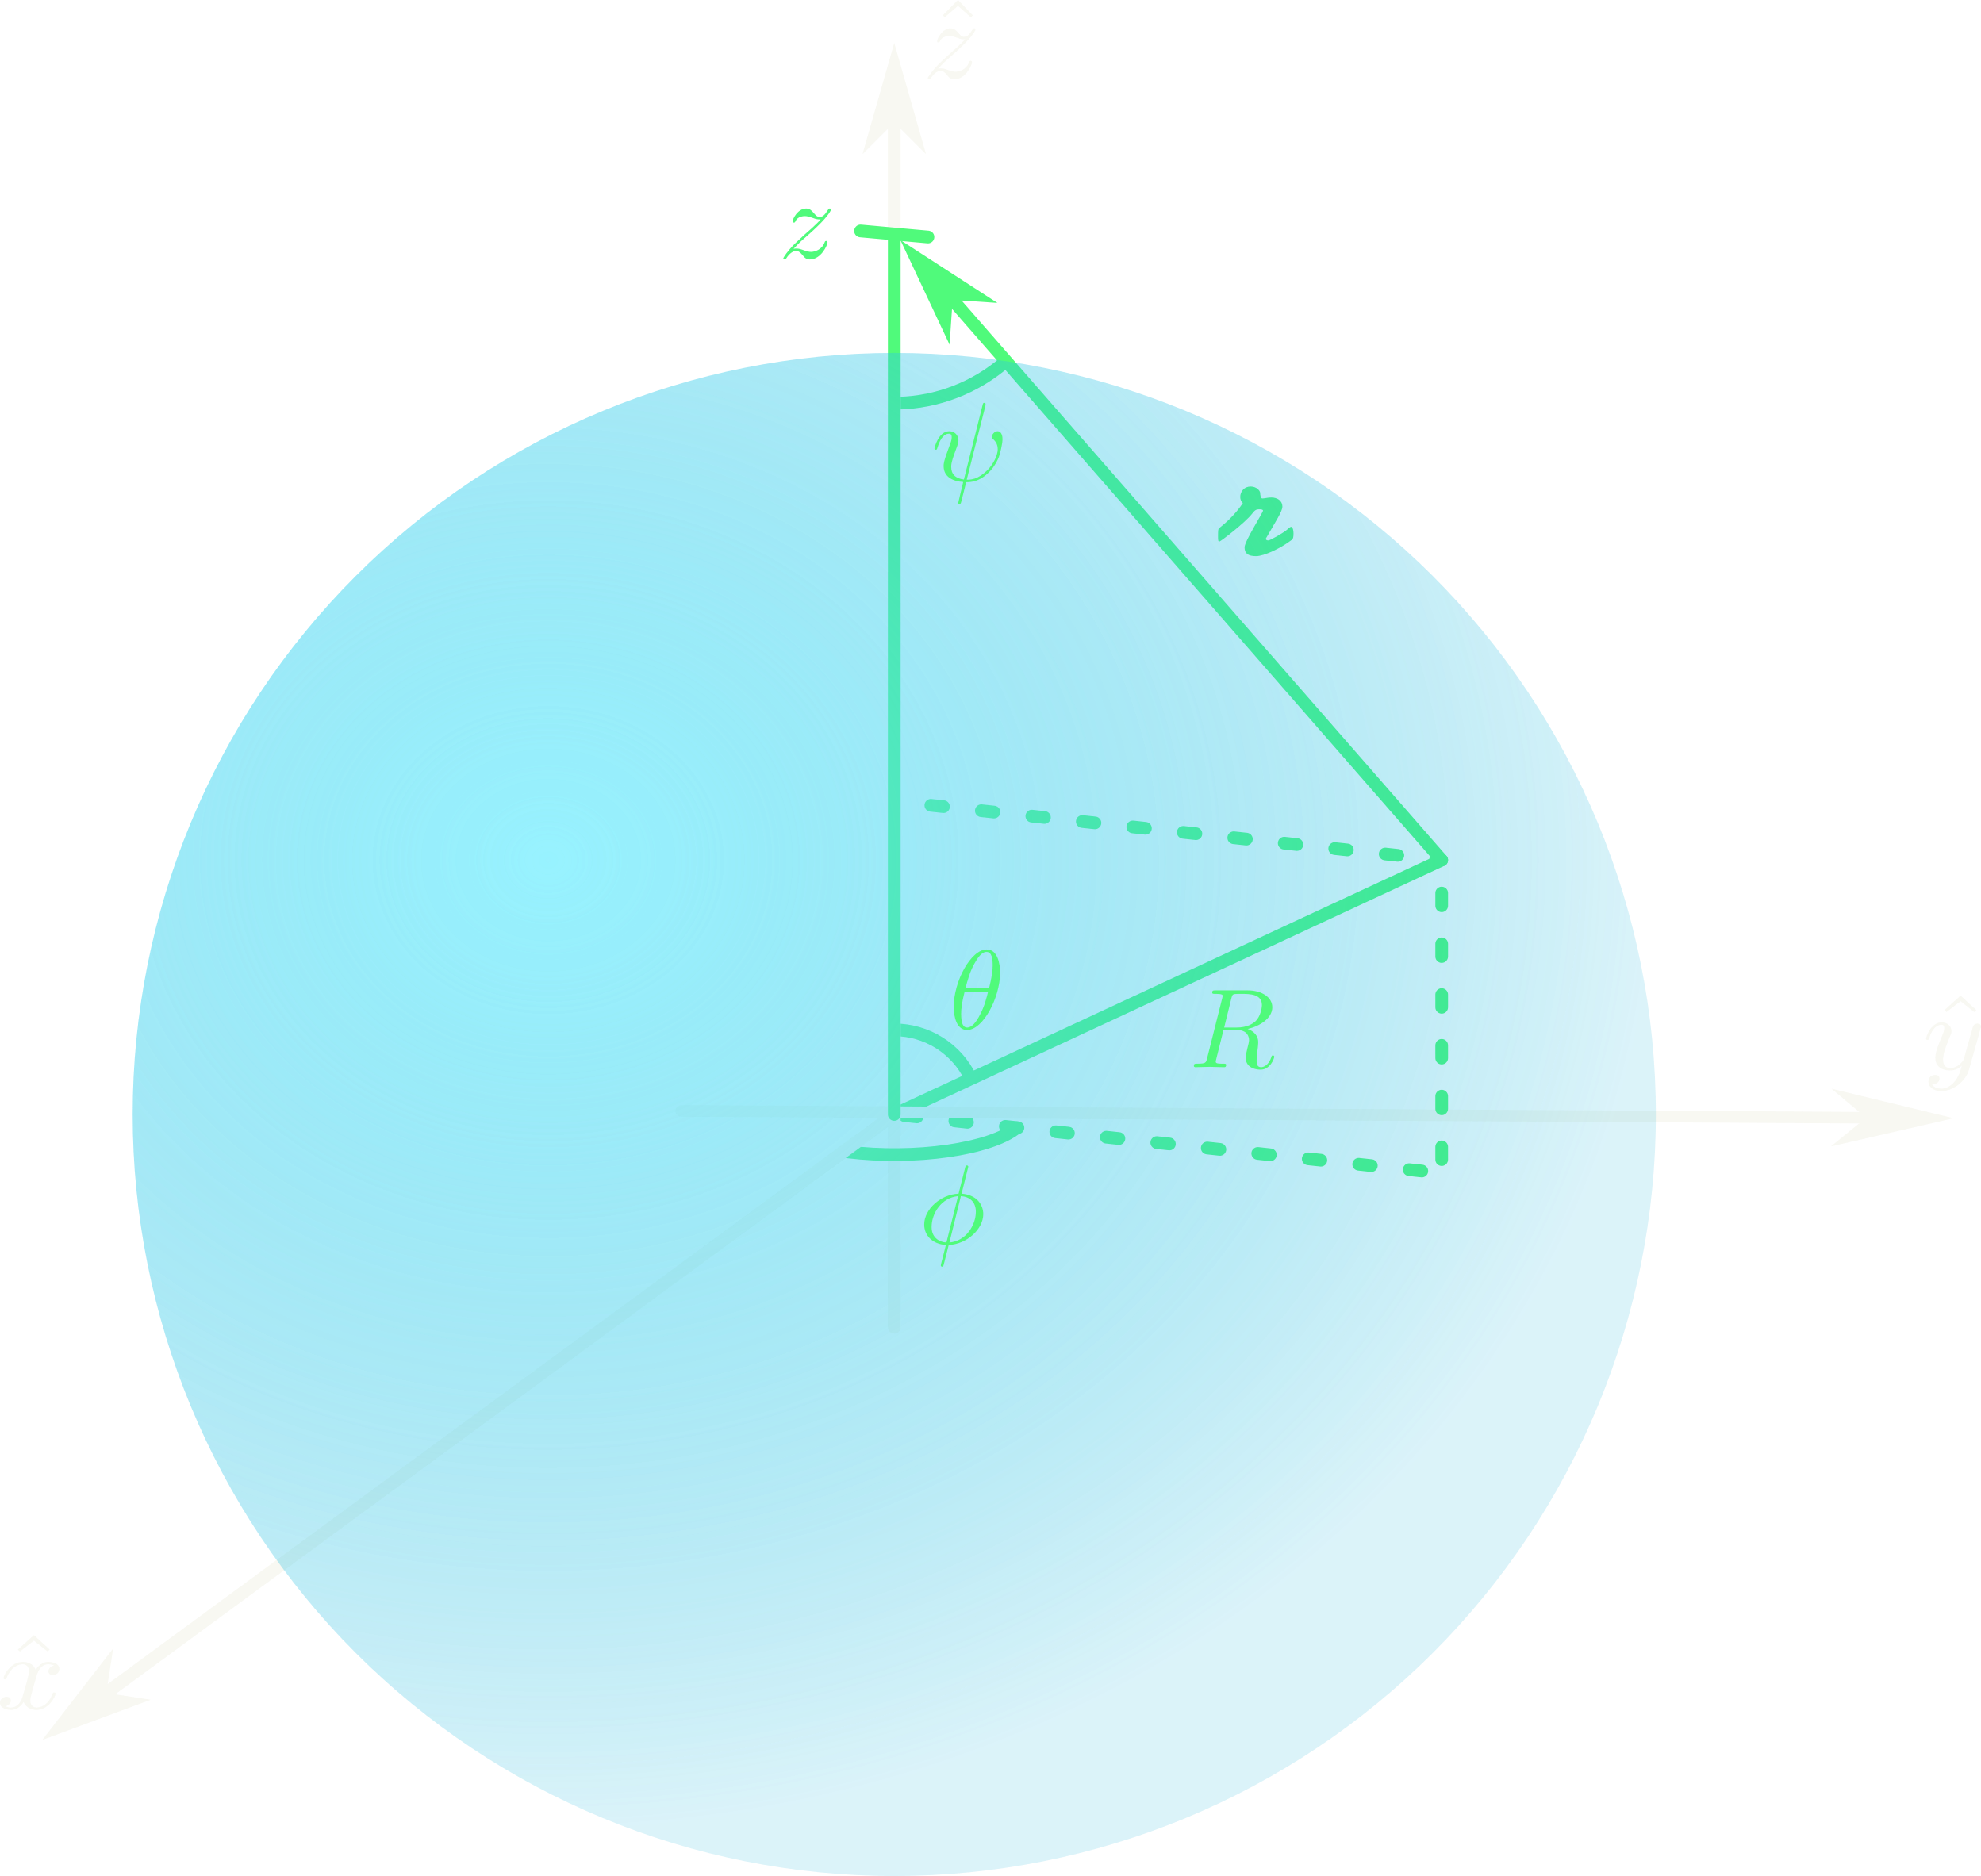
\includegraphics[width=0.5\linewidth]{images/hw2_7.png}
    \captionsetup{width=0.8\linewidth}
    \caption{An electric field a distance $z$ from the center of a spherical surface of radius $R$
    that carries a charge density $\sigma$.}
    \label{fig:2_7}
\end{figure}
Once again, the electric field is in the $z$-direction:
\begin{equation}
    \vb{E} = \frac{1}{4\pi\epsilon_0}   
    \int \frac{\sigma}{\scriptr^2} \cos\psi \vu{z} \dd{\vb{a}}
\end{equation}
From the law of cosines, $\scriptr^2 = z^2 + R^2 - 2zR\cos\theta$; Geometrically,
$\cos\psi = \dfrac{z - R \cos\theta}{\scriptr}$; the surface area element is
$\dd{\vb{a}} = R^2 \sin\theta \dd{\theta} \dd{\theta}$:
\begin{align*}
    \vb{E} &=  \ke\int_0^{2\pi} \int_0^{\pi}
        \frac{\sigma R^2(z - R \cos\theta)}{(z^2 + R^2 - 2zR\cos\theta)^{3/2}}
        \sin\theta \dd{\theta} \dd{\phi} \vu{z} \\
        &= \ke (2\pi\sigma R^2) \int_0^{\pi}
        \frac{z - R \cos\theta}{(z^2 + R^2 - 2zR\cos\theta)^{3/2}}
        \sin\theta \dd{\theta} \vu{z} \\
        &= \ke (2\pi\sigma R^2) f(\theta) \vu{z}
\end{align*}
using the substitution $u = \cos\theta$: $\dd{u} = -\sin\theta \dd{\theta}$, and the limits of
integration are $[\cos{0}, \cos{\pi}]$. So,
\begin{align*}
    f(\theta) =
    \int_{-1}^{1} \frac{z - Ru}{(z^2 + R^2 - 2zRu)^{3/2}} \dd{u} = f(u)
\end{align*}
substituting again with $v = \sqrt{z^2 + R^2 - 2zRu}$; $\dd{v} = -\dfrac{zR}{v} \dd{u}$; and $
u = \dfrac{1}{2zR}(z^2 + R^2 - v^2)$:
\begin{align*}
    f(v) &= -\frac{1}{zR} \int \frac{z - \frac{1}{2z}(z^2 + R^2 - v^2)}{v^3} v \dd{v} \\
    &= -\frac{1}{2z^2R} \int \frac{2z^2 - (z^2 + R^2 - v^2)}{v^2} \dd{v} \\
    &= -\frac{1}{2z^2R} \int \frac{v^2 + z^2 - R^2}{v^2} \dd{v} \\
    &= -\frac{1}{2z^2R} \int \qt(1 + \frac{z^2 - R^2}{v^2}) \dd{v} \\
    &= -\frac{1}{2z^2R} \qt(v - \frac{z^2 - R^2}{v})
\end{align*}
back substituting $v = \sqrt{z^2 + R^2 - 2zRu}$,
\begin{align*}
    f(u) &= -\frac{1}{2z^2R} \qt(\frac{z^2 + R^2 - 2zRu}{\sqrt{z^2+R^2-2zRu}} 
        - \frac{z^2 - R^2}{\sqrt{z^2 + R^2 - 2zRu}}) \eval_{-1}^1 \\
    &= -\frac{1}{2z^2R} \qt(\frac{2R^2 - 2zRu}{\sqrt{z^2+R^2-2zRu}}) \eval_{-1}^1 \\
    &= \frac{1}{z^2} \qt(\frac{zu - R}{\sqrt{z^2+R^2-2zRu}}) \eval_{-1}^1 \\
    &= \frac{1}{z^2} \qt(
        \frac{z - R}{\sqrt{z^2 + R^2 - 2zR}} - \frac{-z - R}{\sqrt{z^2 + R^2 + 2zR}}
    )
\end{align*}
Taking the positive square root: $\sqrt{z^2 + R^2 - 2zR} = (R - z)$ if $R > z$, but $(z - R)$ if
$R < z$. So, for the case $z < R$ (inside the sphere) the electric field is
\begin{align*}
    \vb{E} &= \frac{1}{4\pi\epsilon_0} \frac{2\pi\sigma R^2}{z^2} \qt(
        \frac{z - R}{R - z} - \frac{-z - R}{R + z}
    ) \vu{z} \\
    &= \frac{1}{4\pi\epsilon_0} \frac{2\pi\sigma R^2}{z^2} \qt(
        \frac{z - R}{R - z} + \frac{z + R}{R + z}
    ) \vu{z} \\
    &= \frac{1}{4\pi\epsilon_0} \frac{2\pi\sigma R^2}{z^2} \qt(
        \frac{z - R}{R - z} + 1
    ) \vu{z} \\
    &= \frac{1}{4\pi\epsilon_0} \frac{2\pi\sigma R^2}{z^2} \qt(
        \frac{z - R}{R - z} + \frac{R - z}{R - z}
    ) \vu{z} \\
    &= 0
\end{align*}
For the case $z > R$ (outside the sphere) the electric field is
\begin{align*}
    \vb{E} &= \ke \frac{2\pi\sigma R^2}{z^2} \qt(
        \frac{z - R}{z - R} + \frac{z + R}{z + R}
    ) \vu{z} \\
    &= \ke \frac{4\pi\sigma R^2}{z^2} \vu{z} \\
    &= \ke \frac{q}{z^2} \vu{z}
\end{align*}
This makes sense: From outside the sphere, the point charge $q$ is the
charge-per-area $\sigma$ times the surface area of the sphere $4\pi R^2$, or simply
$q = 4\pi R^2 \sigma$.

\newpage
\paragraph{2.8}\label{hw:2_8}
Finding the field inside and outside a solid sphere of radius $R$ with a uniform volume charge
density $\rho$ is similar to Prob. 2.7. Outside the solid sphere the total charge $q$ contributes
to the electric field as if it were a point charge:
\begin{align*}
    \vb{E}_{out} &= \ke \frac{q}{r^2} \vu{r}
\end{align*}
Inside the solid sphere, only the volume of the solid sphere less than $r$ contributes to the
electric field. The volume of the total sphere is $V = \frac{4}{3}\pi R^3$, and the volume of the
sphere less than $r$ is $V' = \frac{4}{3}\pi r^3$. So, electric field inside the solid sphere is
\begin{align*} 
    \vb{E}_{in} &= \frac{V'}{V} \vb{E}_{out} \\
    &= \frac{r^3}{R^3} \ke \frac{q}{r^2} \vu{r} \\
    &= \ke \frac{q}{R^3} r \vu{r} 
\end{align*}
or
\begin{align*}
    \vb{E}_{in} = \ke \frac{q}{R^3} \vb{r}
\end{align*}
\begin{figure*}[ht]
    \centering
    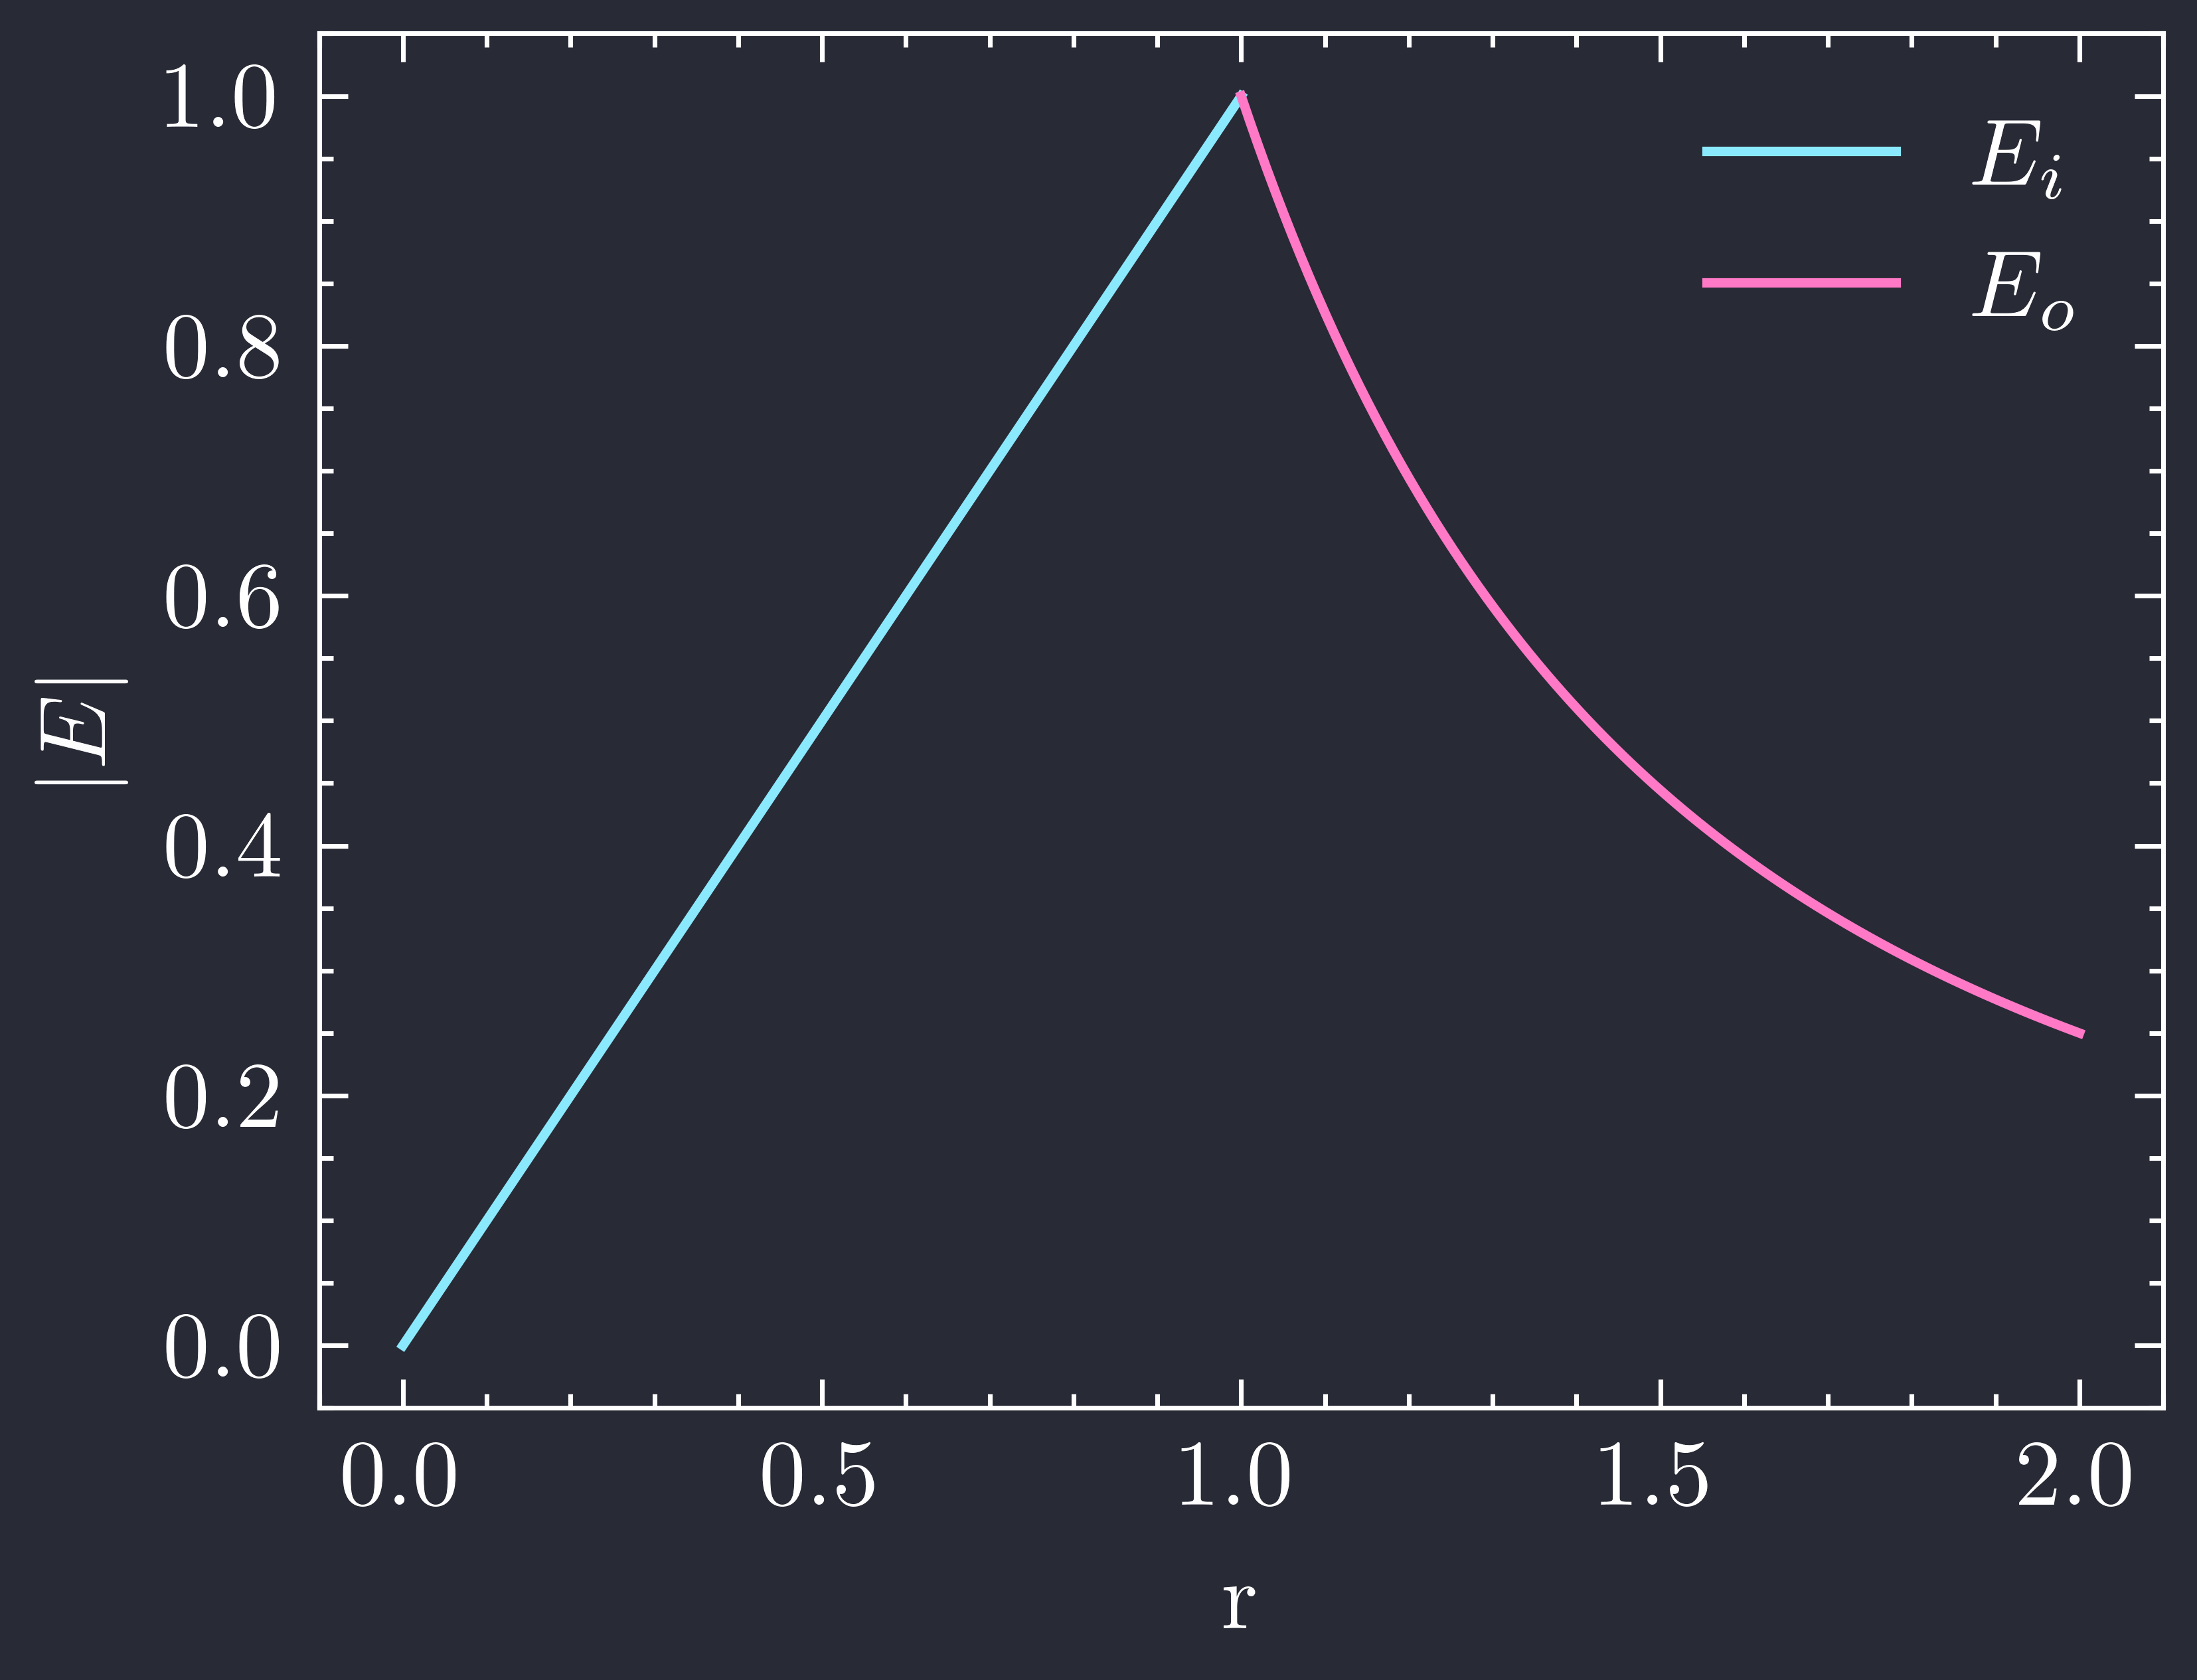
\includegraphics[width=0.8\linewidth]{images/hw2_8.png}
    \captionsetup{width=0.8\linewidth}
    \caption{Magnitude of Electric field $\abs{E}$ as a function of $r$ inside and outside a solid. Where $q = 9$nC and $R = 1$m.}
    \label{fig:2_8}
\end{figure*}
\newpage
\paragraph{2.12}
For a spherical shell of radius $R$ with a uniform surface charge density $\sigma$, the enclosed
charge in side the sphere is $Q_{enc} = 0$, thus the electric field inside the sphere is 
\begin{align*}
    \vb{E}_i = 0
\end{align*}
and using the sphericla symmetry of a Gaussian surface, the electric field outside the sphere is
\begin{align*}
    \oint \vb{E}_o \vdot \dd{\vb{a}} &= \frac{1}{\epsilon_o} Q_{enc} \\
    \abs{\vb{E}_0} \int \dd{\vb{a}} &= \frac{1}{\epsilon_o} (4\pi\sigma R^2) \\
    \vb{E}_o (4\pi r^2) &= \frac{1}{\epsilon_o} (4\pi\sigma R^2) \vu{r} \\
    \vb{E}_o &= \frac{\sigma R^2}{\epsilon_o r^2} \vu{r}
\end{align*}

\newpage
\paragraph{2.16} \label{hw:2_16}
A thick spherical shell with charge density
\begin{align*}
    \rho = \frac{k}{r^2} \quad (a\leq r \leq b)
\end{align*}
The electric field in the three regions: \\
(i) \(r<a\)
\[ Q_{enc} = 0; \vb{E} = 0 \]

(ii) \(a\leq r \leq b\)
\[ Q_{enc} = \int_0^{2\pi} \int_0^\pi \int_a^r \rho (r^2 \sin\theta) \dd{r} \dd{\theta} \dd{\phi}
= 4\pi \int_a^r \frac{k}{r^2} (r^2) \dd{r} = 4\pi k (r - a) \]
And from Gauss's law,
\begin{align*}
    \oint \vb{E} \vdot \dd{\vb{a}} &= \frac{1}{\epsilon_o} Q_{enc} \\
    \abs{\vb{E}} \int \dd{a} &= \frac{1}{\epsilon_o} 4\pi k (r - a) \\
    E (4\pi r^2) &= \frac{1}{\epsilon_o} 4\pi k (r - a)
\end{align*}
or 
\begin{align*}
    \vb{E} &= \frac{k (r - a)}{\epsilon_o r^2} \vu{r} = \ke \frac{4\pi k(r - a)}{r^3} \vb{r}
\end{align*}

(iii) \(r>b\)
\[ Q_{enc} = \int_0^{2\pi} \int_0^\pi \int_a^b \rho (r^2 \sin\theta) \dd{r} \dd{\theta} \dd{\phi}
= 4\pi k (b - a) \]
And from Gauss's law,
\begin{align*}
    \oint \vb{E} \vdot \dd{\vb{a}} &= \frac{1}{\epsilon_o} Q_{enc} \\
    \abs{\vb{E}} \int \dd{a} &= \frac{1}{\epsilon_o} 4\pi k (b - a) \\
    E (4\pi r^2) &= \frac{1}{\epsilon_o} 4\pi k (b - a)
\end{align*}
or
\begin{align*}
    \vb{E} &= \frac{k (b - a)}{\epsilon_o r^2} \vu{r} = \ke \frac{4\pi k(b - a)}{r^3} \vb{r}
\end{align*}
\begin{figure}[ht]
    \centering
    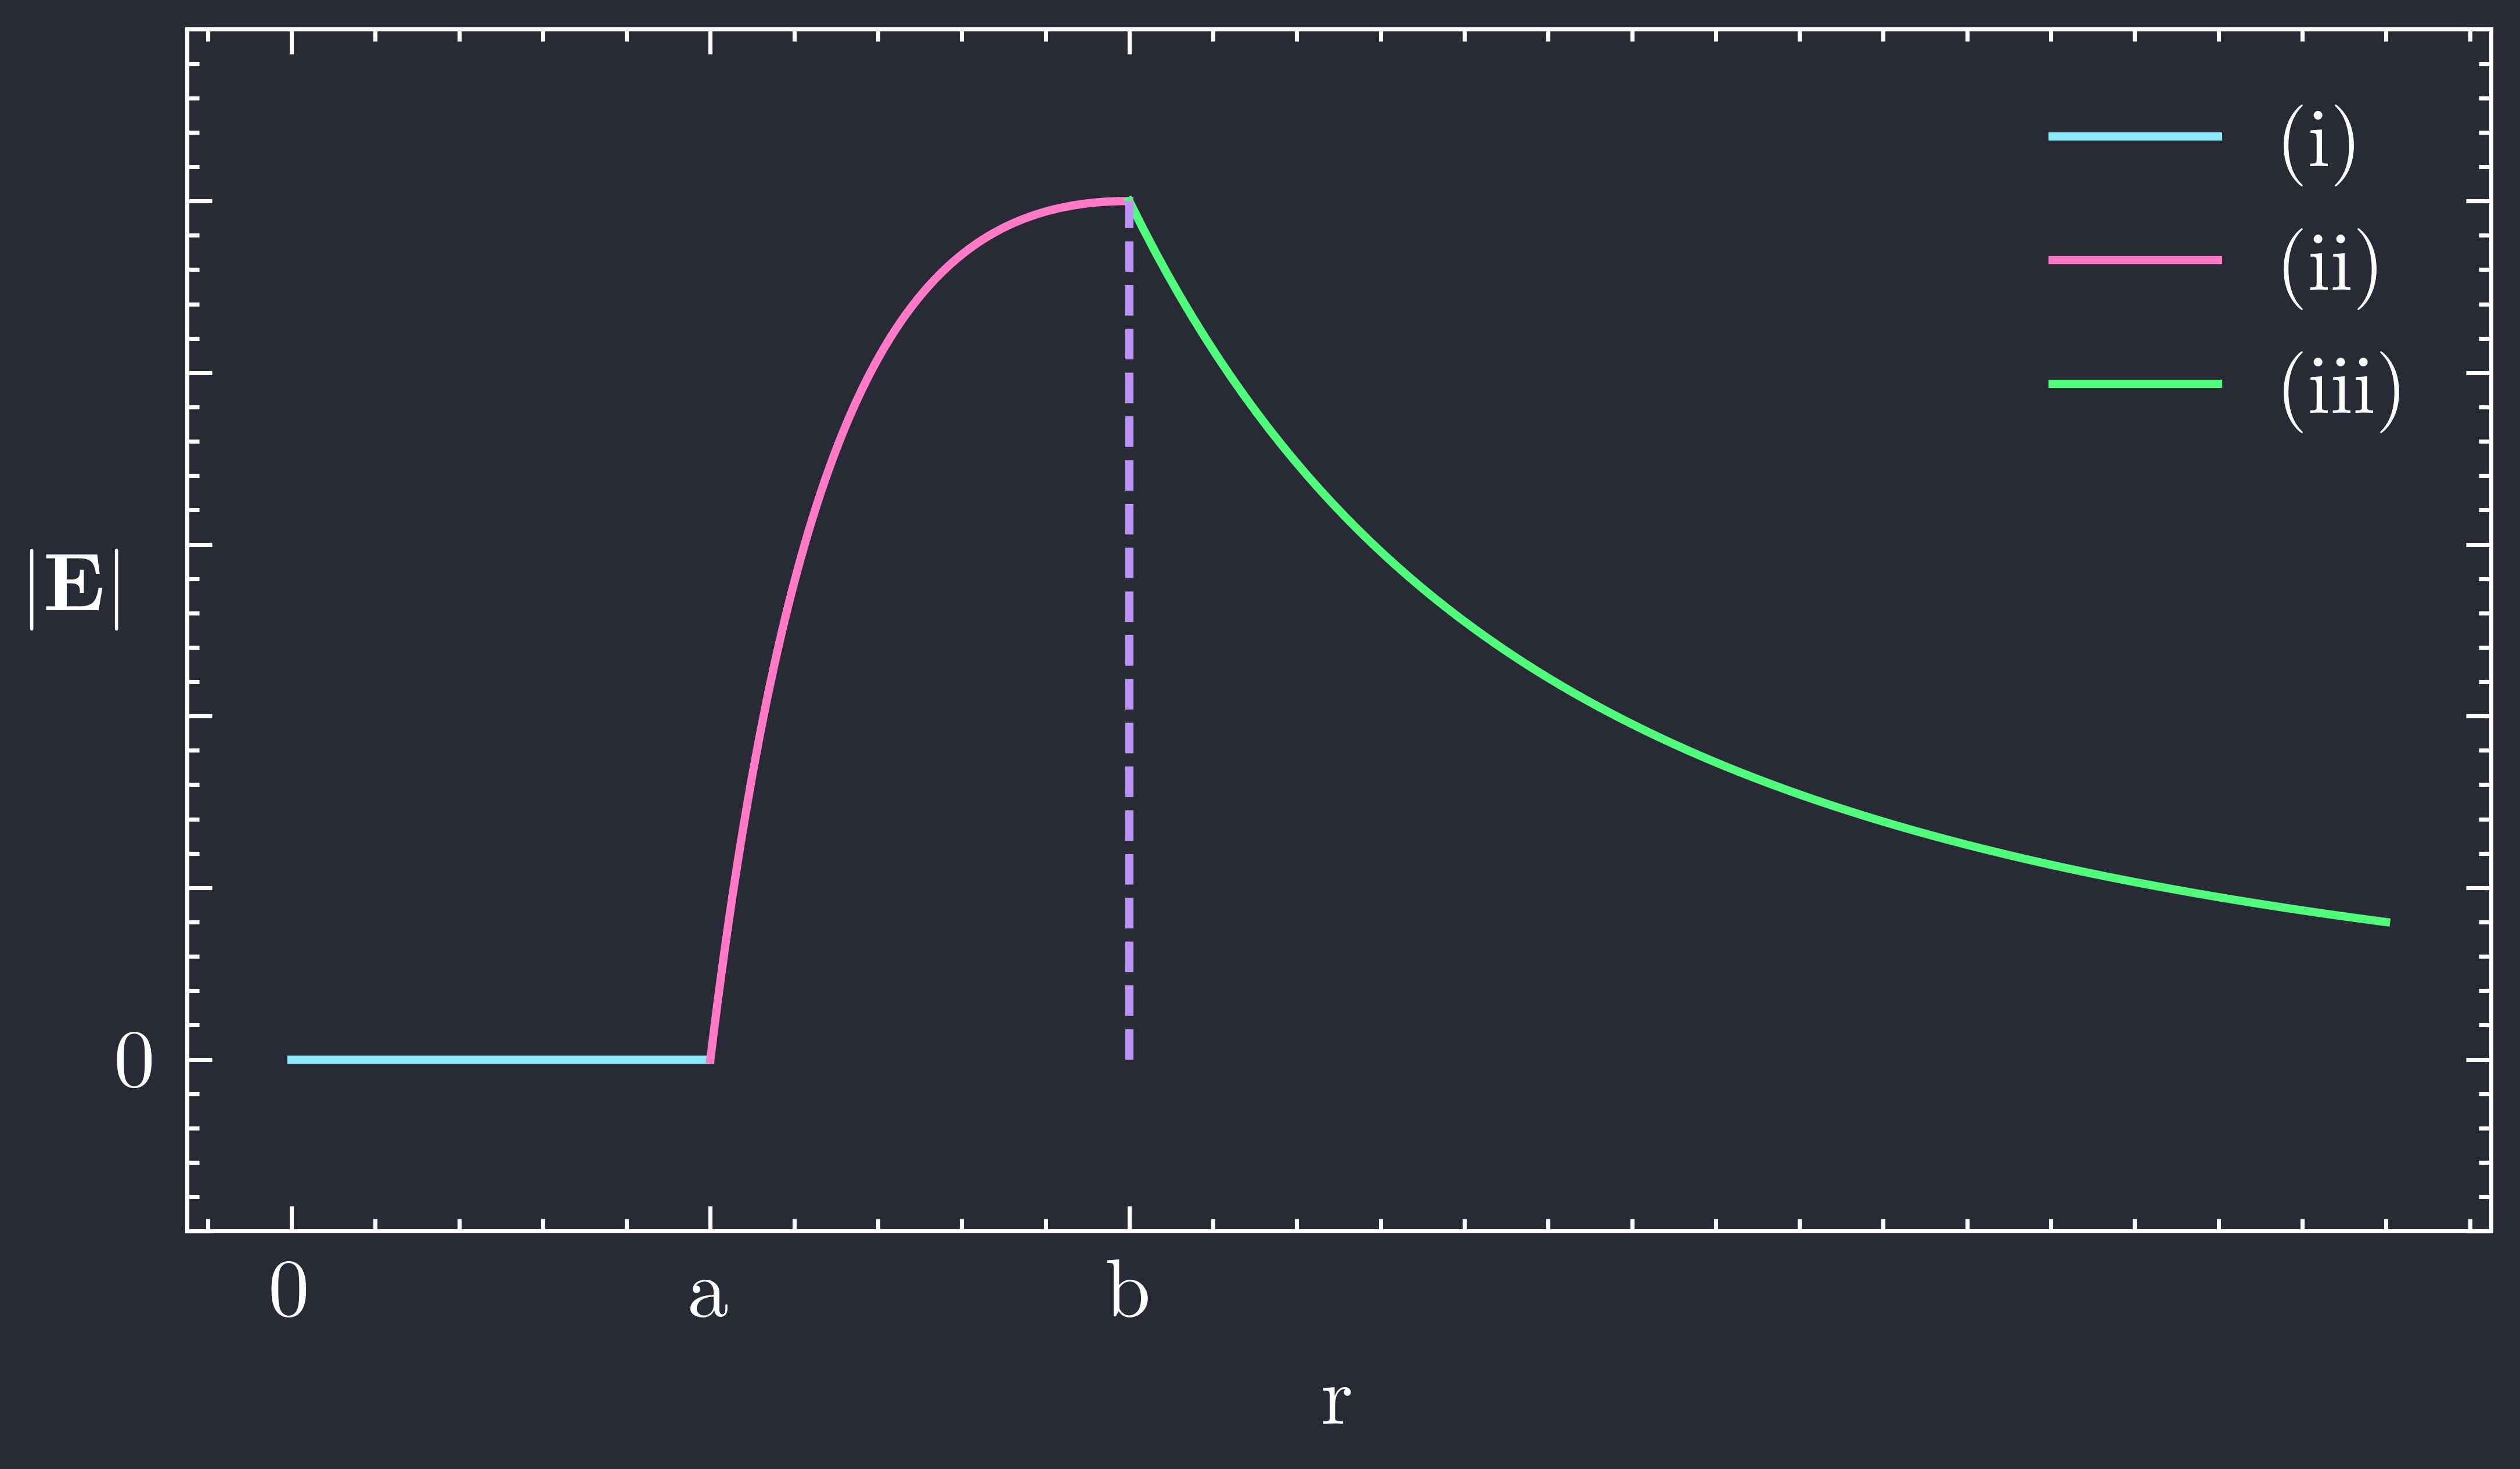
\includegraphics[width=0.8\linewidth]{images/hw2_15.png}
    \captionsetup{width=0.8\linewidth}
    \caption{Plot of $\abs{\vb{E}}$ as a function of $r$, for the case $b = 2a$.}
    \label{fig:2_15}
\end{figure}

\clearpage
\newpage
\paragraph{2.18}
Finding the electric field, as a function of $y$, where $y=0$ is the center of an infinite plane
slab, of thickness $2d$, carrying a uniform volume charge density $\rho$. For the case \(y > 2d\)
The enclosed charge is
\begin{align*}
    Q_{enc} = \rho (2d) A = 2\rho Ad
\end{align*}
where $A$ is the area of the Gaussian pillbox. Using Gauss's law,
\begin{align*}
    \oint \vb{E} \vdot \dd{\vb{a}} &= \frac{1}{\epsilon_o} Q_{enc} \\
    \abs{\vb{E}} \int \dd{a} &= \frac{1}{\epsilon_o} 2\rho Ad \\
    E (2A) &= \frac{1}{\epsilon_o} 2\rho Ad \\
    \vb{E} &= \frac{\rho d}{\epsilon_o} \vu{y}
\end{align*}
For the case \(0 < y < 2d\), the enclosed charge is
\begin{align*}
    Q_{enc} = 2\rho y A
\end{align*}
and the electric field is
\begin{align*}
    E (2A) &= \frac{1}{\epsilon_o} \rho y A \\
    \vb{E} &= \frac{\rho y}{\epsilon_o} \vu{y}
\end{align*}
In the $-y$ direction, $E$ is negative as shown in Figure \ref{fig:2_17}.
\begin{figure}[ht]
    \centering
    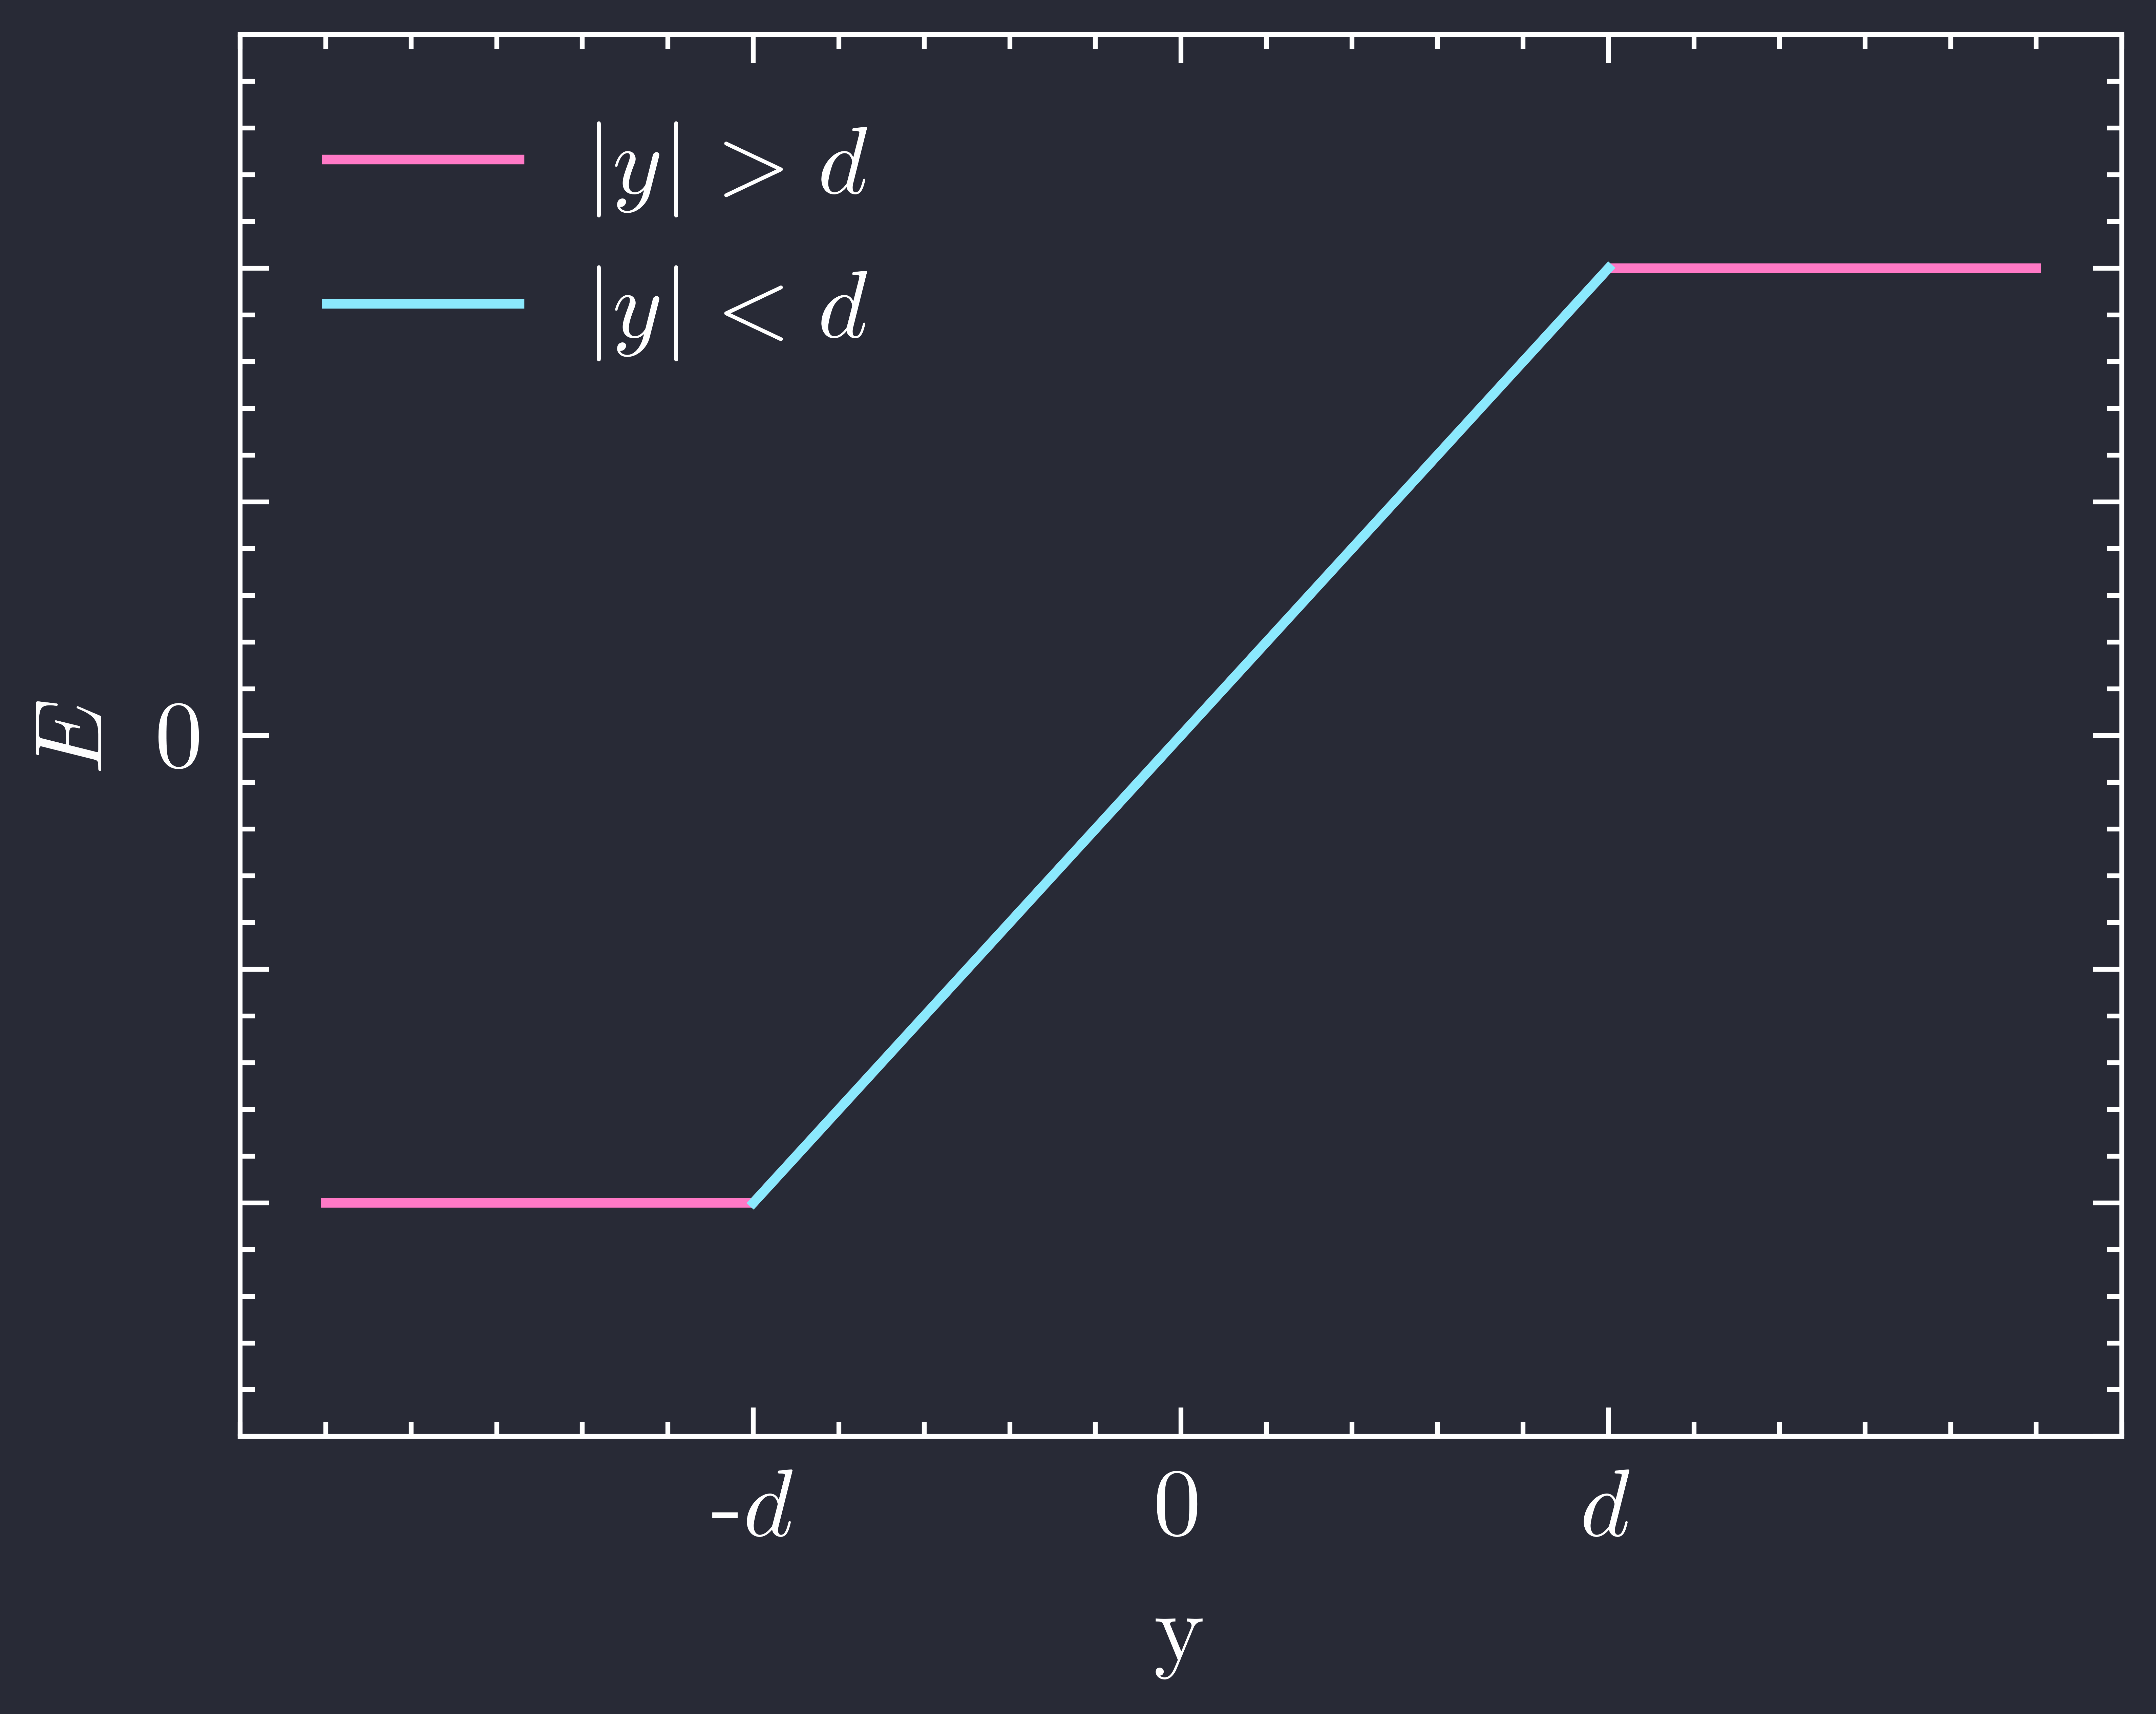
\includegraphics[width=0.8\linewidth]{images/hw2_17.png}
    \captionsetup{width=0.8\linewidth}
    \caption{Plot of $\abs{\vb{E}}$ as a function of $y$}
    \label{fig:2_17}
\end{figure}

\end{document}